\chapter{Flash-Speicher\label{chapter:flash}}
\lhead{Flash-Speicher}
\begin{refsection}
\chapterauthor{Roger Billeter und Gabriel Looser}

\section{Allgemeines zu Flash-Speichern}
\rhead{Allgemeines zu Flash-Speichern}
Der Flash-Speicher ist ein elektrisches Speicherelement, welches
weit verbreitet ist.
Das Ziel ist ein einfaches Modell f"ur den Schreib- und Lesevorgang
n"aherzubringen.

\subsection{Floating Gate Transistor}
\rhead{Floating Gate Transistor}
Floating Gate Transistoren z"ahlen zu den Feldeffekttransistoren
(Siehe Abbildung \ref{skript:Floatinggatetransistor}).
Im Floating Gate wird die Ladung gespeichert, aus dem man einen Bin"aren
Zustand bestimmen kann.
Je nach Ladungsmenge im Floating Gate k"onnen auch mehrere Bits gespeichert
werden, "ublicherweise werden jedoch 2 Bits in einem Floating Gate
Transistor gespeichert.
Die Ladung im Floating Gate l"asst sich "uber das Control Gate steuern.
Wird das Potential am Control Gate erh"oht, beginnt von Drain nach
Source ein Strom zu fliessen.
Somit fliessen nun in der n"ahe des Floating Gates Elektronen durch.
"Ublicherweise wird der Source Anschluss meistens mit GND verbunden und
Drain wird beim Leseprozess auf 0V geh"angt und beim Schreibprozess
"ublicherweise auf "uber 10V.

\begin{figure}
\centering
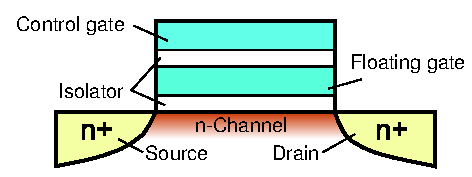
\includegraphics[width=0.7\textwidth]{flash/graphics/Floatinggate.pdf}
\caption{Abbildung eines Floting Gate Transistor \cite{flash:floatinggate}}
\label{skript:Floatinggatetransistor}
\end{figure}

\subsection{Flash-Typen}
\rhead{Flash-Typen}
Bei den Flash-Speichern wird zwischen zwei Typen unterschieden, den NAND
und den NOR Typen.
Diese unterscheiden sich in der Zusammenschaltung der einzelnen Transistoren.

\subsubsection{NAND Typ}
\rhead{NAND Typ}
Bei einem NAND Flash-Speicher werden die einzelnen Transistoren zu einer
NAND Speicherzelle zusammen geschaltet.
Die Speicherzellen werden in Gruppen in Serie geschaltet.
Die Speicherzellengruppe teilt sich eine Datenleitung, daher muss das
Lesen und Schreiben immer in der ganzen Gruppe sequentiell erfolgen.
Dadurch wird die Anzahl Datenleitungen reduziert und der Flash-Speicher
ben"otigt weniger Platz.
NAND Flash-Speicher haben ihre Verwendung vor allem in Bereichen, wo viel
Speicher m"oglichst wenig Platz brauchen darf und die Zugriffszeit keine
grosse Rolle spielt.
Verwendung finden sie vor allem in USB-Sticks, Flash-Speicherkarten
(z.B. SD-Speicherkarten) und als Speicher in MP3-Playern.

\subsubsection{NOR Typ}
\rhead{NOR Typ}
Bei einem NOR Flash-Speicher werden die Transistoren zu einer NOR
Speicherzelle zusammen geschaltet.
Die Speicherzellen werden "uber die Datenleitungen parallel geschaltet,
dadurch kann auf jede Speicherzelle direkt zugegriffen werden.
Die Parallelleitungen brauchen mehr Platz, es lassen sich jedoch k"urzere
Zugriffszeiten realisieren.
Die NOR Flash-Speicher finden z.B. bei Programmspeichern und Firmwarespeichern
ihre verwendung.

\subsection{L"oschvorgang}
\rhead{Lo"schvorgang}
Der L"oschvorgang kann erreicht werden, indem das Potential am 
Control Gate heruntergesetzt wird.
So wird erreicht, dass es zum Tunneleffekt kommt und die Ladung fliesst
aus dem Floating Gate ab.
Alles zum Tunneleffekt kann im Kapitel \ref{tunnel:tunneleffekt} nachgelesen werden.

\subsection{Schreibvorgang und Zyklenzahl}
\rhead{Schreibvorgang und Zykklenzahl}
F"ur den Speichervorgang m"ussen Elektronen mittels 'hot electron injection'
in das Floating-Gate gebracht werden. Ein grosses Problem bei
Flashspeichern ist die begrenzte Anzahl Schreibezyklen.
Wegen dem Schreibvorgang mittels 'hot electron injection', wird die
Oxidschicht (Isolation \ref{skript:Floatinggatetransistor}) um das Floating Gate herum
besch"adigt, da bei der 'hot electron injection' eine grosse Leistung
ben"otigt wird.
Dies bewirkt, dass durch die Oxidschicht immer mehr Ladung abfliessen kann.
Bei den NOR-Flashs hat man etwa 10'000 bis 100'000 Zyklen.
Hingegen bei den NAND-Flashs sind es doch gegen 2 Millionen Zyklen.
Da der Speicher jedoch in einzelnen Bl"ocken aufgebaut ist, ist dies
eher ein kleines Problem.
Wenn eine Zelle ausf"allt hat es immer noch gen"ugend andere, auch wenn
dadurch immer ein bisschen an Speicher verloren geht.

\section{Modell f"ur den Schreibvorgang}
\subsection{Modell des Potentialtopfs und der Anregung}
\rhead{Modell des Potentialtopfs und der Anregung}
F"ur den Floating Gate Transistor wird ein vereinfachtes Modell
gew"ahlt um die Funktionsweise und die Berechnung besser zu illustrieren.
Als Modell f"ur das Floating-Gate wird ein Potentialtopf verwendet,
in dem die Elektronen gespeichert werden.
Als Vereinfachung des Schreibvorgangs kann man sich das Putten beim
Golf vorstellen.
Das Elektron ist der Golfball und der Potentialtopf das Loch (Siehe Abbildung \ref{skript:Minigolf}).
Das Elektron landet jedoch nicht, wie der Golfball, wegen der Schwerkraft
im Potentialtopf, sondern es gibt Energie ab an den Potentialtopf und
wird dadurch abgebremst.
Wird das Elektron stark genug abgebremst, landet es im Potentialtopf.

\begin{figure}
\centering
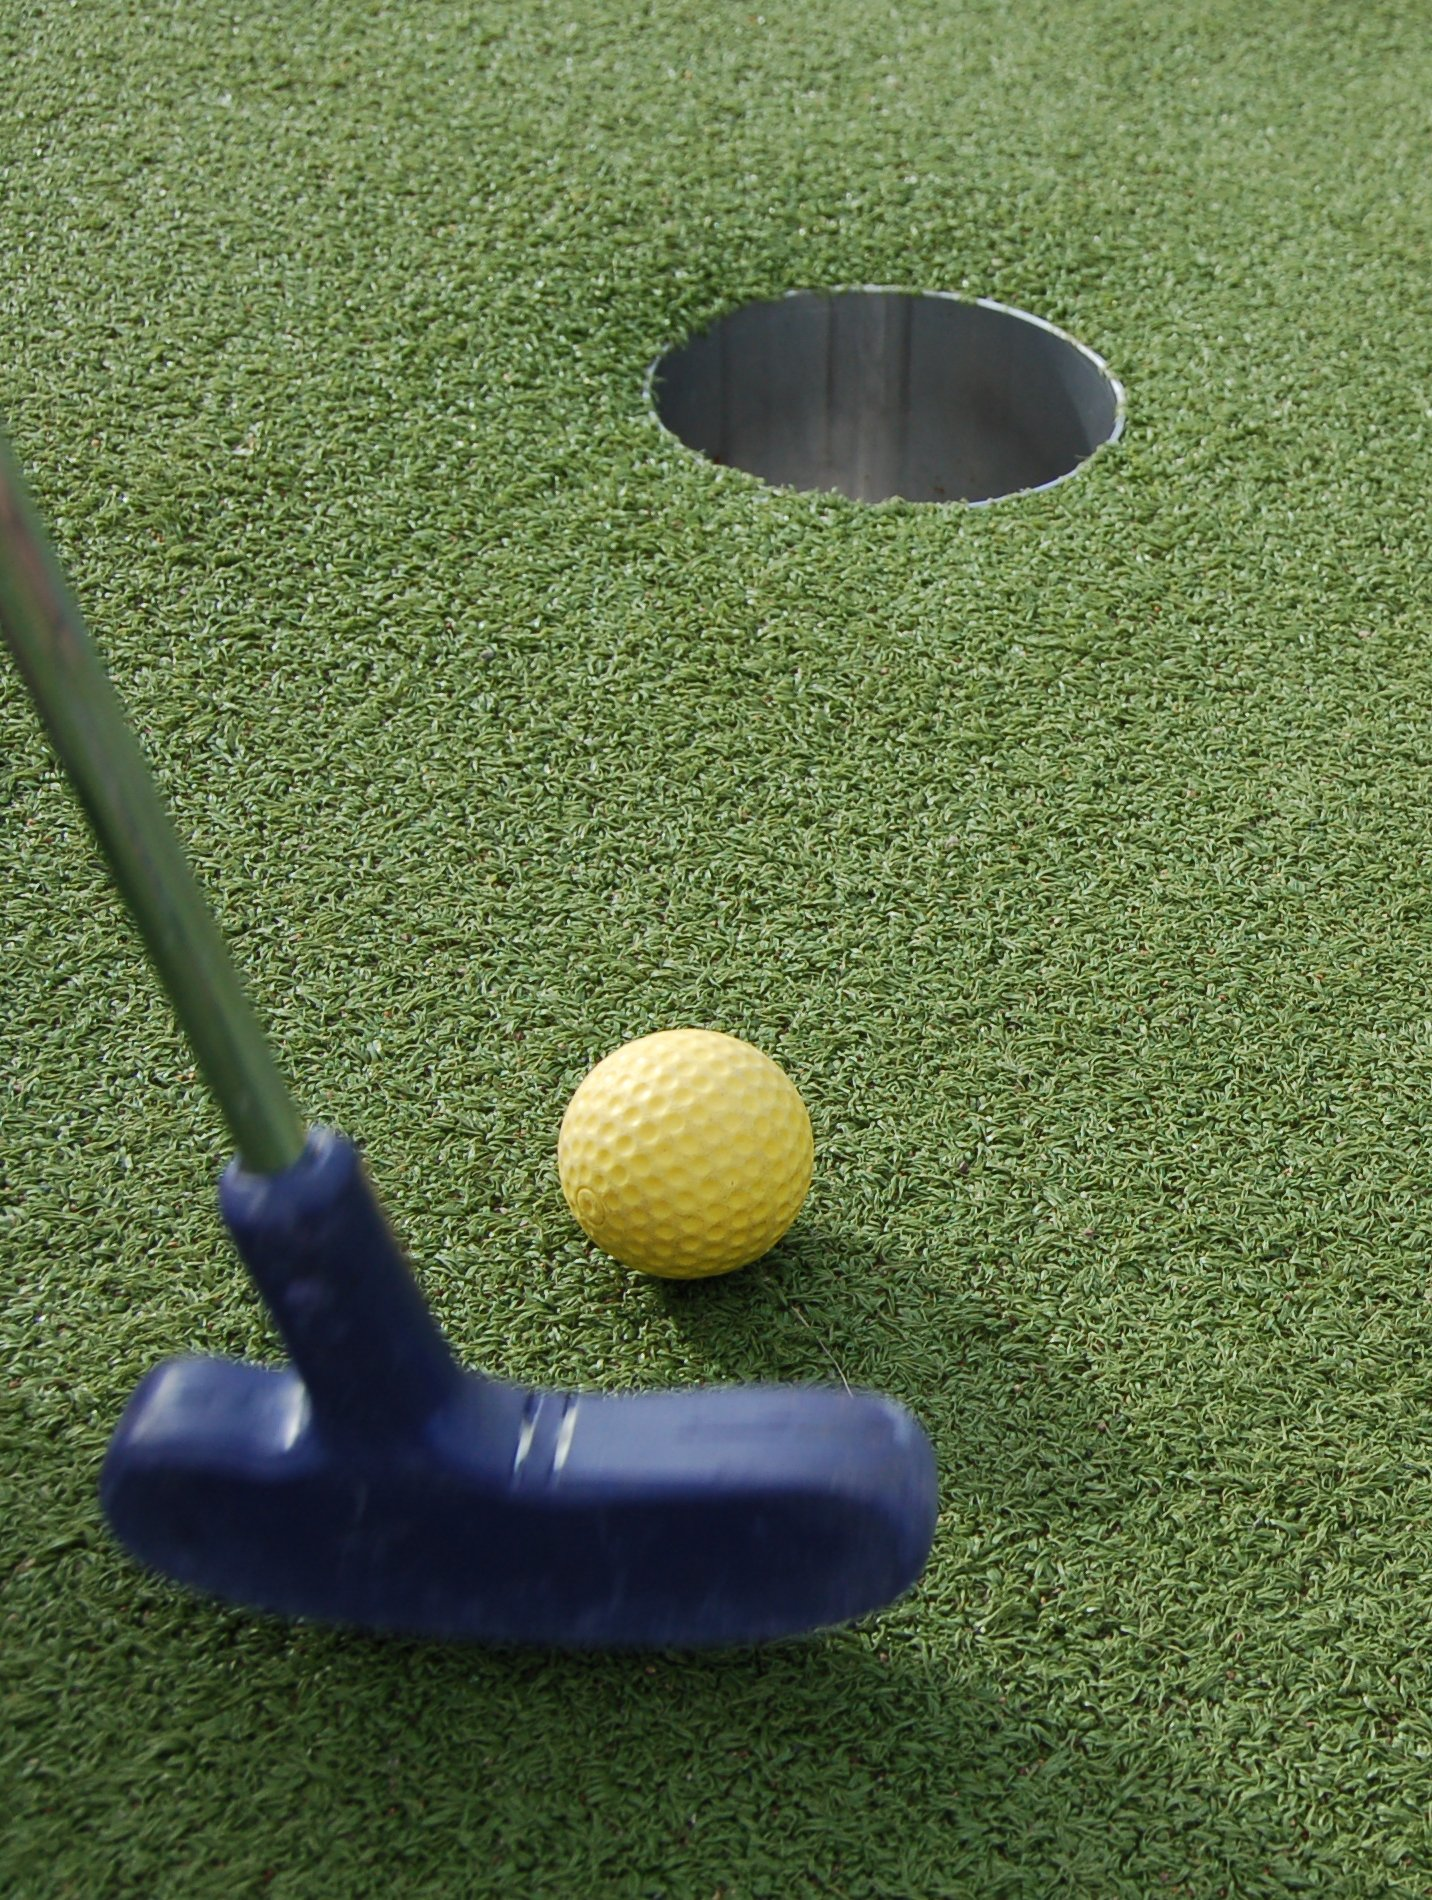
\includegraphics[width=0.3\textwidth]{flash/graphics/Minigolf.jpg}
\caption{Abbildung Minigolf mit Loch \cite{flash:golf}
\label{skript:Minigolf}}
\end{figure}

Am Anfang befindet sich im Potentialtopf Teilchen im Grundzustand $|0\rangle$
mit der Grundenergie $E_{0}$.
Das vorbeifliegende Elektron hat eine h"ohere Energie und st"ort mit
einem Potential $V_{e}(x,t)$ (Siehe Abbildung \ref{flash:Anregung})
den Potentialtopf.
Die Teilchen bremsen das Elektron ab und nehmen Energie auf, dadurch
wird die Energie $E_{0}$ gr"osser und es kommt zu einem "Ubergang 
zwischen dem Zustand $|0\rangle$ und dem Zustand $|1\rangle$.
Die Teilchen im Potentialtopf k"onnten nat"urlich noch mehr Energie
absorbieren, indem sie zu einem Zustand $|2\rangle$ mit noch h"oherer
Energie "ubergehen, doch wegen der h"oheren Energiedifferenz ist dieser
"Ubergang weniger wahrscheinlich.
Auf die Berechung der Wahrscheinlichkeit mit mehr als zwei Zust"anden
wir verzichtet, da dies nur ein Modell sein soll.

Die Teilchen im Potentialtopf haben Energien, welche den jeweiligen 
Wellenfunktionen entsprechen.
Als Vereinfachung dieser Grundschwingung dient die Vorstellung eines
Wackelpuddings, welcher durch das vorbei fliegende Elektron zus"atzlich
in Schwingung versetzt wird, indem das Elektron einen Druck auf den
Wackelpudding aus"ubt.
Das Grundpotential wird asymmetrisch angeregt.
Wenn man dies auf das Modell des Wackelpudding "ubertr"agt, erkennt man,
dass wenn man einen Wackelpudding gleichm"assig zusammendr"uckt, wird
dieser nicht zus"atzlich in Schwingung versetzt.
Wird der Wackelpudding jedoch auf der einen Seite angestossen, wird der
Wackelpudding zus"atzlich in Schwingung versetzt und erreicht ein
h"oheres Energieniveau.
F"ur die Berechnung wird der Potentialtopf "uber die h"alfe mit einem
Rechteckimpuls angeregt.
Dies vereinfacht das L"osen der Differentialgleichungen.
Da die L"osung der urspr"unglichen Gleichung auf ein partielles
Differential-Gleichungssystem f"uhrt und da das L"osen partieller
Differentialgleichungen nicht Stoff des Bachelorstudiums ist, werden
die Gleichungen mittels Skalarpordukt auf ein normales
Differential-Gleichungssystem vereinfacht.

Schlussendlich wird die Wahrscheinlichkeit des Zustand $|0\rangle$ 
respektive die Wahrscheinlichkeit des Zustand $|1\rangle$ errechnet.
Steigt die Wahrscheinlichkeit des Zustand $|1\rangle$ sinkt gleichzeitig
die Wahrscheinlichkeit des Zustand $|0\rangle$ und umgekehrt.
Diese Wahrscheinlichkeit ist abh"angig von der Energie $V_{e}$ 
des Elektrons, vom Abstand $(x)$ des Elektrons zum Potentialtopf und der 
Geschwindigkeit respektive der Zeit $(t)$ mit der das Elektron auf den 
Potentialtopf wirkt.

\begin{figure}
\centering
\includegraphics{flash/potential-1.pdf}
\caption{St"orpotential f"ur das Modell f"ur den Schreibprozess bei
einem Flashspeicher
\label{flash:Anregung}}
\end{figure}

\subsection{"Ubergangswahrscheinlichkeit}
\rhead{"Ubergangswahrscheinlichkeit}
Es wird die Wahrscheinlichkeit errechnet mit der die Teilchen
vom Grundzustand $|0\rangle$ in den Zustand $|1\rangle$ wechseln
und damit Energie aufnehmen. 
Diese Wahrscheinlichkiet ist $\vert\langle1|\psi(t)\rangle\vert^2$
daher muss zuerst $\langle1|\psi(t)\rangle$ berechnet werden.

\subsection{L"osung der Schr"odingergleichung}
\rhead{L"osung der Schr"odingergleichung}
Die Schr"odingergleichung ergibt sich aus der kinetischen Energie des
Potentialtopfes und der potentiellen Energie der Anregung.
Mit der Schr"odingergleichung wird nicht die Energie der Elektronen
sondern die Energie der Teilchen berechnet.
\[
i\hbar\frac{d}{dt}|\psi(t)\rangle = H|\psi(t)\rangle = \Bigg{(}-\frac{\hbar^2}{2m} \frac{\partial^2}{\partial x^2}+V(x)+V_{e}(x,t)\Bigg{)}|\psi(t)\rangle
\]

Wenn man den Zustand nun von 0 auf 1 erh"oht sieht dies folgendermassen aus:
\[
i\hbar\frac{d}{dt}\langle1|\psi(t)\rangle = \Bigg{\langle}1\Bigg{|}-\frac{\hbar^2}{2m} \frac{\partial^2}{\partial x^2}+V(x)+V_{e}(x,t)\Bigg{|}\psi(t)\Bigg{\rangle}
\]

Was nun genauer ausgerechnet wird ist $\langle1|\psi(t)\rangle$, denn
dies entspricht der Wahrscheinlichkeit, dass der $|1\rangle$ erreicht ist.

Wenn man die Gleichung nun noch vereinfacht, sieht man, dass diese
Wahrscheinlichkeit mehrfach vorkommt.
\[
i\hbar\frac{d}{dt}\langle1|\psi(t)\rangle = E_{1}\langle1|\psi(t)\rangle+\langle1|\psi(t)\rangle V(t)
\]

Das Ganze kann man nun auch mit dem Zustand $|0\rangle$ machen. Diese
Gleichung sieht sehr "ahnlich aus.
\[
i\hbar\frac{d}{dt}\langle0|\psi(t)\rangle = E_{0}\langle0|\psi(t)\rangle+\langle0|\psi(t)\rangle V(t)
\]

\subsection{Skalarprodukt}
\rhead{Skalarprodukt}

Mittels Skalarprodukt kann das Differentialgleichungssystem weiter
vereinfacht werden.
Denn wie man weiss ergibt das Skalarprodukt von $\langle0|0\rangle$
und $\langle1|1\rangle = 1$.
Genauso wie das Skalarprodukt von $\langle0|1\rangle$ und
$\langle1|0\rangle = 0$.
Ausserdem kann  $\langle0|V(t)|0\rangle$ als $V_{0}v_{00}$ geschrieben
werden, $\langle1|V(t)|0\rangle$ als $V_{0}v_{01}$,$\langle0|V(t)|0\rangle$
als $V_{0}v_{11}$ und $\langle1|V(t)|0\rangle$ als $V_{0}v_{10}$.

Einfachheitshalber schreibt man anstatt $\langle1|\psi(t)\rangle$ $a_1$
entsprechend f"ur $\langle0|\psi(t)\rangle$ $a_0$.
Somit ergibt sich dann folgendes Differentialgleichungssystem:
\begin{align*}
i\hbar\frac{d}{dt}a_{0}(t)\langle0|0\rangle +i\hbar\frac{d}{dt}a_{1}(t)\langle0|1\rangle&= a_{0}(t)E_{1}\langle0|0\rangle + a_{1}(t)E_{1}\langle0|1\rangle + a_{0}(t)\langle0|V(t)|0\rangle+ a_{1}(t)\langle1|V(t)|0\rangle
\\
i\hbar\frac{d}{dt}a_{0}(t)\langle1|0\rangle +i\hbar\frac{d}{dt}a_{1}(t)\langle1|1\rangle&= a_{0}(t)E_{1}\langle1|0\rangle + a_{1}(t)E_{1}\langle1|1\rangle + a_{0}(t)\langle0|V(t)|0\rangle+ a_{1}(t)\langle1|V(t)|0\rangle
\end{align*}
Daraus folgt:
\begin{align}
i\hbar\dot{a}_0&= (E_{0} + V_{0} v_{00}) a_{0} + V_{0} v_{01} a_{1}
\\
i\hbar\dot{a}_1&= V_{0} v_{10} a_{0} + (E_{1} V_{0} v_{11}) a_{1}
\end{align}

\subsection{Variation der Konstanten}
\rhead{Variation der Konstanten}
Die L"osung der Differentialgleichung oszilliert schnell, da die
Frequenz der Gundschwingung sehr gross ist.
Diese Oszillation kann jedoch heraus gefiltert werden, indem man die
Konstanten variiert.
Das Prinzip der Variation der Konstanten wird an folgendem Beispiel
illustriert.
Die Konstanten entsprechen der Energien und der Potentiale, welche nun
Zeitabh"angig gemacht werden.
\[
\dot{a} = C a(t) + D(t) \Rightarrow a(t) = k(t) e^{C t}
\] 
durch ableiten und das einsetzen von $ a(t)$ und  $ \dot{a} $ erhalten wir:

\[
k'(t) e^{C t} + C k(t) e^{C t} = C k(t) e^{C t} + D(t)
\] 
Hier k"urzt sich $ C k(t) e^{C t} $ heraus und somit ist der schnell
oszillierende Teil ist weg.
Daraus folgt:
\[
k'(t) = D(t) e^{-C t}
\] 
integriert diese Gleichung nach der Zeit folgt:
\[
k(t) = \int D(t) e^{-C t} dt 
\]

\subsection{Variation der Konstanden f"ur zwei Differentialgleichungen}
\rhead{Variation der Konstanden f"ur zwei Differentialgleichungen}
Angewandt auf das Differentialgleichungssystem,
wobei $C_{00}$ $(E_{0} + V_{0} v_{00})$
entspricht,
$C_{01}$ $V_{0} v_{01}$,
$C_{10}$ $V_{0} v_{10}$ und $C_{11}$ $(E_{1} V_{0} v_{11})$:
\begin{align*}
\dot{a_{0}}(t) &= C_{00}a_{0}(t) + C_{01}a_{1}(t)
\\
\dot{a_{1}}(t) &= C_{10}a_{0}(t) + C_{11}a_{1}(t)
\end{align*}

Wenn $ C_{01}$ und $ C_{10}$ $ =0$ dann w"are die L"osung:
\begin{align*}
a_{0}(t)&= k_0 e^{C_{00} t} 
\\
a_{1}(t)&= k_1 e^{C_{11} t}
\end{align*}
Wenn die Konstanten $ k_0 $ und $ k_1 $
auch von der Zeit abh"angig sind, ist die L"osung: 
\begin{align*}
a_{0}(t)&= k_0(t) e^{C_{00} t} 
\\
a_{1}(t)&= k_1(t) e^{C_{11} t} 
\end{align*}
Eingesetzt in das Differentialgleichungssystem folgt daraus:
\begin{align*}
k'_{0}(t) e^{C_{00} t} + k_{0}(t) C_{00} e^{C_{00} t}&= k_{0}(t) C_{00} e^{C_{00} t} + k_{1}(t)C_{01}e^{C_{11} t}
\\
k'_{1}(t) e^{C_{11} t} + k_{1}(t) C_{11} e^{C_{11} t}&= k_{0}(t) C_{10} e^{C_{00} t} + k_{1}(t)C_{11}e^{C_{11} t}
\end{align*}
Gemeinsame Terme werden heraus gek"urzt, daraus folgt:
\begin{align*}
k'_{0}(t) e^{C_{00} t}&= k_{1} C_{01} e^{C_{11} t}
\\
k'_{1}(t) e^{C_{11} t}&= k_{0} C_{10} e^{C_{00} t}
\end{align*}
Diese Gleichungen nach $ k'_{0}(t)$ und $ k'_{1}(t)$ aufgel"ost ergibt:
\begin{align*}
k'_{0}(t)&= k_{1}(t) C_{01} e^{(C_{11}-C_{00}) t}
\\
k'_{1}(t)&= k_{0}(t) C_{10} e^{(C_{00}-C_{11}) t}
\end{align*}
Unsere inhomogene Differential-Gleichung erster Ordnung verwandelt
sich dadurch in eine homogene Differential-Gleichung zweiter Ordnung.
\begin{align*}
k''_{0}(t) - (C_{11}-C_{00}) k'_{0}(t) - C_{10}C_{01}k(t)&= 0
\\
k''_{1}(t) - (C_{00}-C_{11}) k'_{1}(t) - C_{01}C_{10}k(t)&= 0
\end{align*}
Das charakteristische Polynom lautet:
\begin{align*}
\lambda_{0}^{2} - (C_{11}-C_{00})\lambda_{0} - C_{10}C_{01}&= 0
\\
\lambda_{1}^{2} - (C_{00}-C_{11})\lambda_{1} - C_{01}C_{10}&= 0
\end{align*}
Die $ \lambda $ der ersten Gleichung lauten:
\[
\lambda_{1,2} = \frac{(C_{11}-C_{00})\pm \sqrt{(C_{11}-C_{00})^2-4(C_{10}C_{01})}}{2}
\]
Die $ \lambda $ der zweite Gleichung lauten:
\[
\lambda_{3,4} = \frac{(C_{00}-C_{11})\pm \sqrt{(C_{00}-C_{11})^2-4(C_{01}C_{10})}}{2}
\]
Nun kann man die $\lambda$ wieder in das charakteristische Polynom
einsetzen und numerisch berechnen lasen, dazu kann zum Beispiel Matlab
verwendet werden.

\begin{figure}
\centering
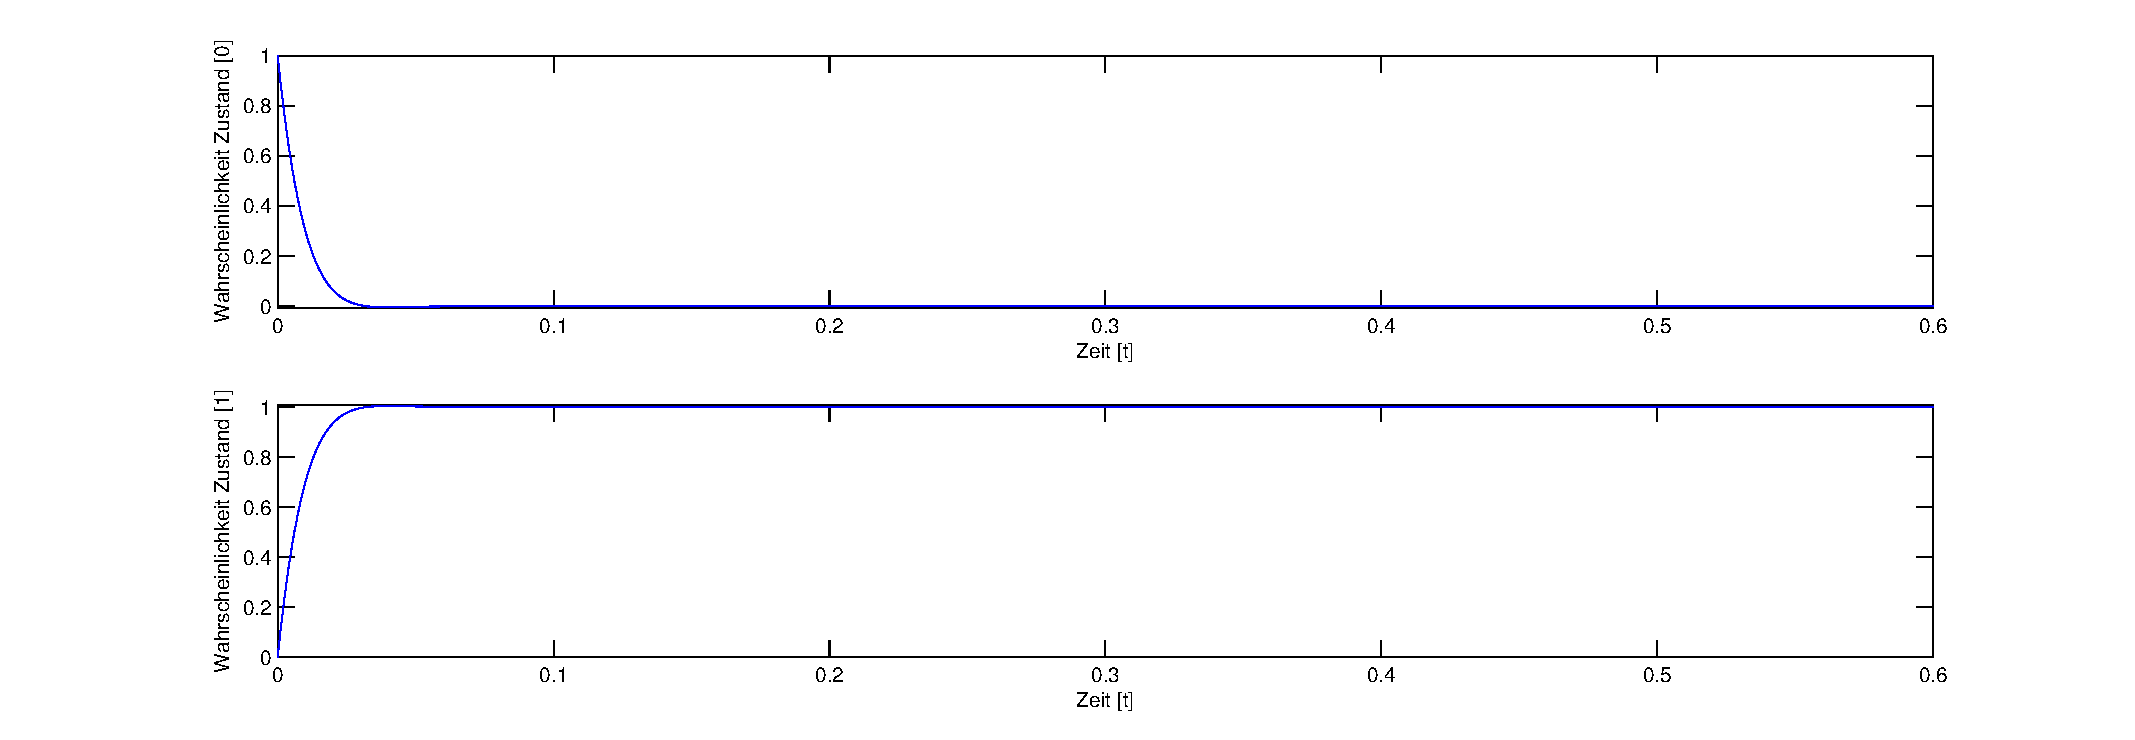
\includegraphics[width=1\textwidth]{flash/graphics/potentialmittel.pdf}
\caption{Abbildung: Wahrscheinlichkeit mit mittlerem Anregungspotential
\label{skript:potentialmittel}}
%
\centering
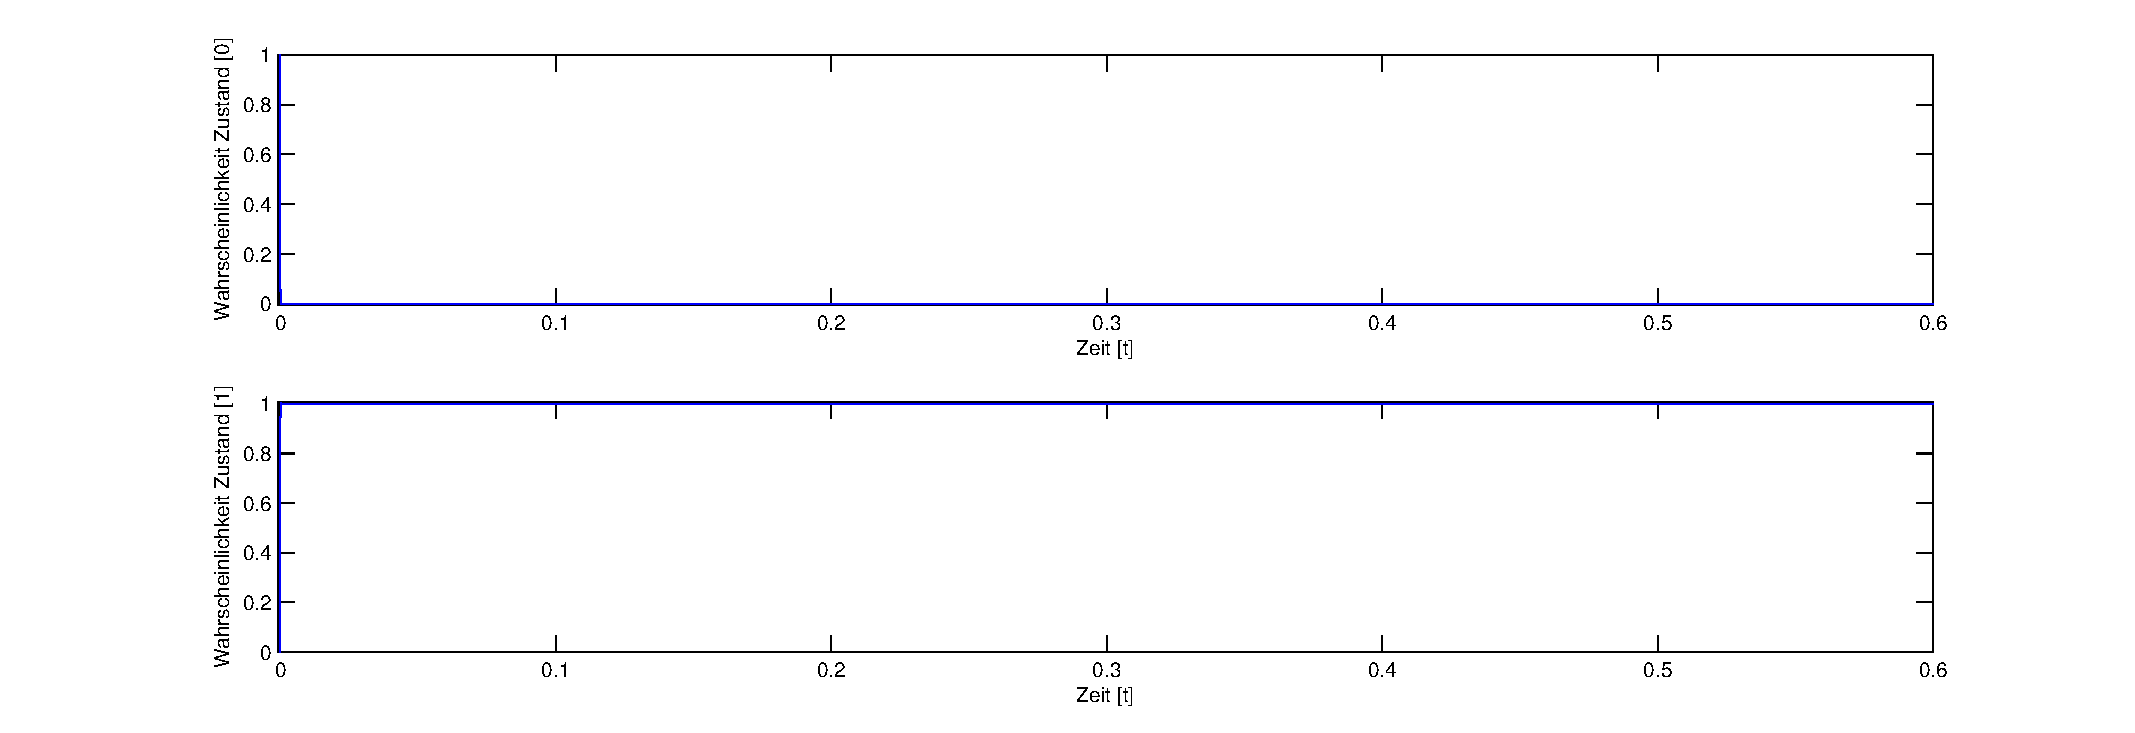
\includegraphics[width=1\textwidth]{flash/graphics/potentialgross.pdf}
\caption{Abbildung:Wahrscheinlichkeit mit 50-Fach gr"osserem Anregungspotential
\label{skript:potentialgross}}
%
\centering
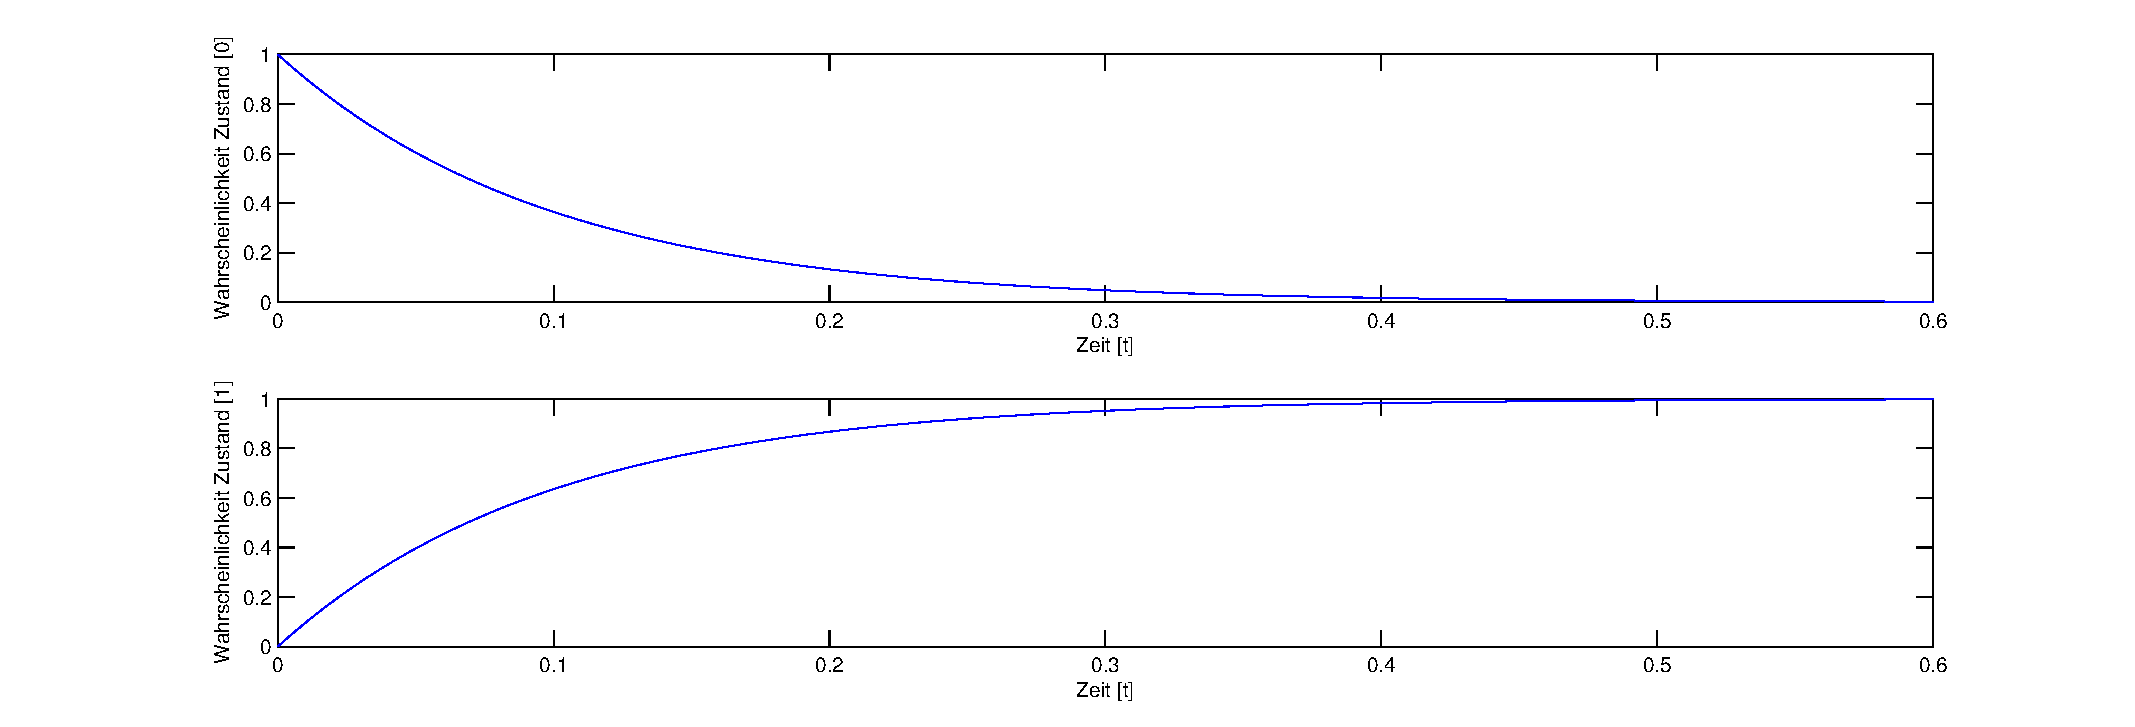
\includegraphics[width=1\textwidth]{flash/graphics/potentialklein.pdf}
\caption{Abbildung:Wahrscheinlichkeit mit 30-Fach kleinerem Anregungspotential
\label{skript:potentialklein}}
\end{figure}

\subsection{Numerische Resultate}
\rhead{Numerische Resultate}
In der Abbildung \ref{skript:potentialmittel}, sieht man in der unteren
Grafik, dass man nach ca. 0.02s sagen kann das der Zustand $|0\rangle$, 
respektive in der oberen Grafik der Zustand $|1\rangle$ erreicht wird.
Wenn man das Potential um das 50-Fache erh"oht, sieht man in der Abbildung
\ref{skript:potentialgross}, dass die Wahrscheinlichkeit, f"ur  den Zustand
$|0\rangle$ viel schneller kleiner wird und die Wahrscheinlichkeit f"ur den
Zustand $|1\rangle$ viel schneller ansteigt.
Wenn man jedoch das Potential um das ca. 30-Fache verkleinert, dauert es
um einiges l"anger bis die Wahrscheinlichkeit, dass der Zustand $|0\rangle$,
wie in Abbildung \ref{skript:potentialklein} zu sehen ist, erreicht wird,
respektive bis die Wahrscheinlichkeit, dass der Zustand $|1\rangle$ erreicht
wird.

Das Modell zeigt, dass die Teilchen im Potentialtopf dem vorbeifliegenden
Elektron Energie entziehen und es abbremsen k"onnen.
Im realen Halbleiter sind die Teilchen Wellen im Elektronengas,
sogenannte Plasmonen.


\printbibliography[heading=subbibliography]
\end{refsection}
